\section{The parser}

So far the parser takes cml files (version 2008-->2010) and works with Firefox and Internet Explorer.\\
N.B: Javascript does not conveniently work with file input stream, so the most convenient way to deal with it is to:

(i)   Make a string out of the cml file.

(ii)  Load the cml string into an XML object.

(iii) Parse the object and extract the information we want to create the metaSpecObject

\subsection{A few points}
Before rendering everything, some things have to be done
\subsubsection{SetCoordinatesWithPixel}
The file contains relative coordinates, that is, they need to be transfomed into actual coordinates in order to be properly rendered.
This is done in the method setCoordinateWithPixel:
    \begin{figure}[h]
    \begin{centering}
    \caption{The object Peak}
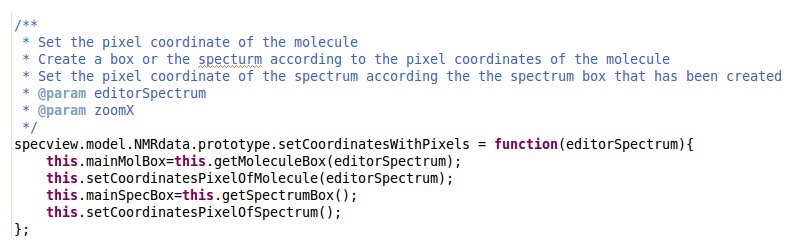
\includegraphics[width=195mm,height=55mm]{./images/setCoordinatesWithPixel}
%    \label{subd}
    \end{centering}
    \end{figure}
That method is an instance method of the metaSpecObject. The first step is to define:

(i) Get the molecule box where the molecule will be drawn.

(ii) Set the pixel coordinates of the molecule.

(iii) Set the spectrum box according to the molecule box.

(iv) Set the pixel coordinates of the spectrum(e.g of all the peaks)
\\

\textbf{Get the molecule box}

    \begin{figure}[h]
    \begin{centering}
    \caption{Get the molecule box}
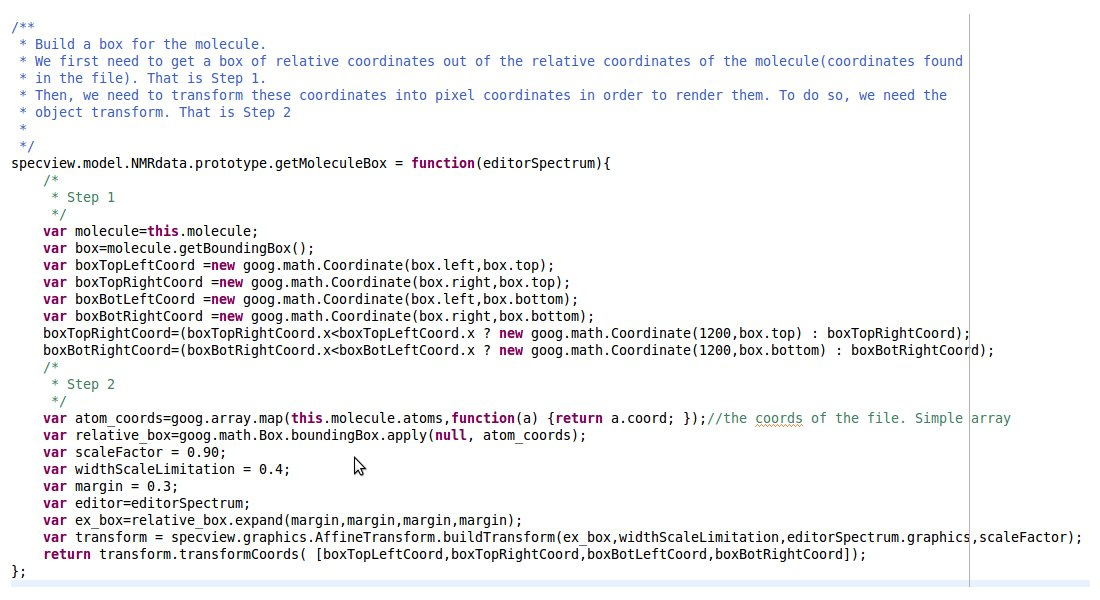
\includegraphics[width=195mm,height=100mm]{./images/getMoleculeBox}
%    \label{subd}
    \end{centering}
    \end{figure}

The method take as an input the editor object, and return an array of 4 coordinates (pixel coordinates) that will be used to draw the molecule box.

\textbf{Transform object}

In order to transform relative coordinates into actual coordinates, we need to take into account the dimension(e.g width andheight) of the canvas editor (which is an attribute of the editor object). This is the reason why the method has an input ``editorSpectrum'' which is the editor object. This is used in the method to create a ``transform'' object which does the transformation from realtive coordinates into actual coordinates.
\clearpage
\textbf{Set the molecule coordinates}

    \begin{figure}[h]
    \begin{centering}
    \caption{Set the molecule Coordinates}
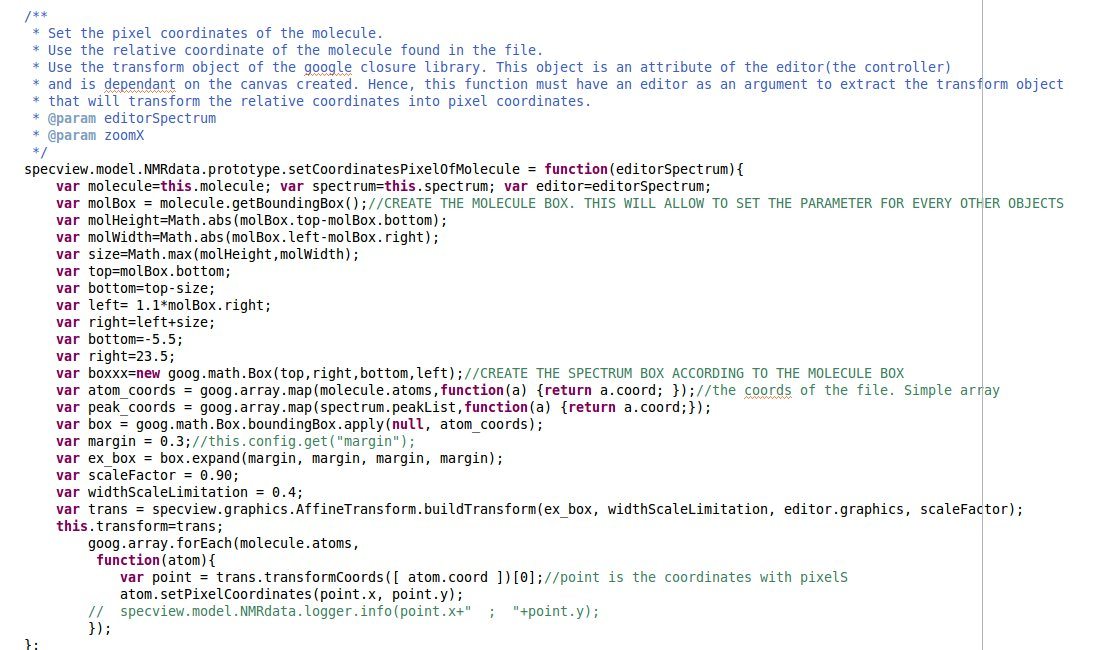
\includegraphics[width=195mm,height=120mm]{./images/setMoleculeCoordinates}
%    \label{subd}
    \end{centering}
    \end{figure}
\clearpage
\textbf{Get the spectrum box}
    \begin{figure}[h]
    \begin{centering}
    \caption{Get the spectrum box}
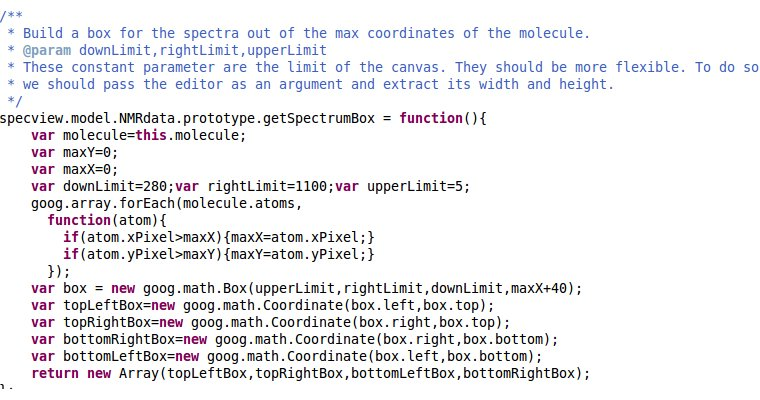
\includegraphics[width=155mm,height=68mm]{./images/getSpecBox}
%    \label{subd}
    \end{centering}
    \end{figure}
\textbf{Set the spectrum pixel coordinates}
    \begin{figure}[h]
    \begin{centering}
    \caption{Set the pixel coordinates pixel}
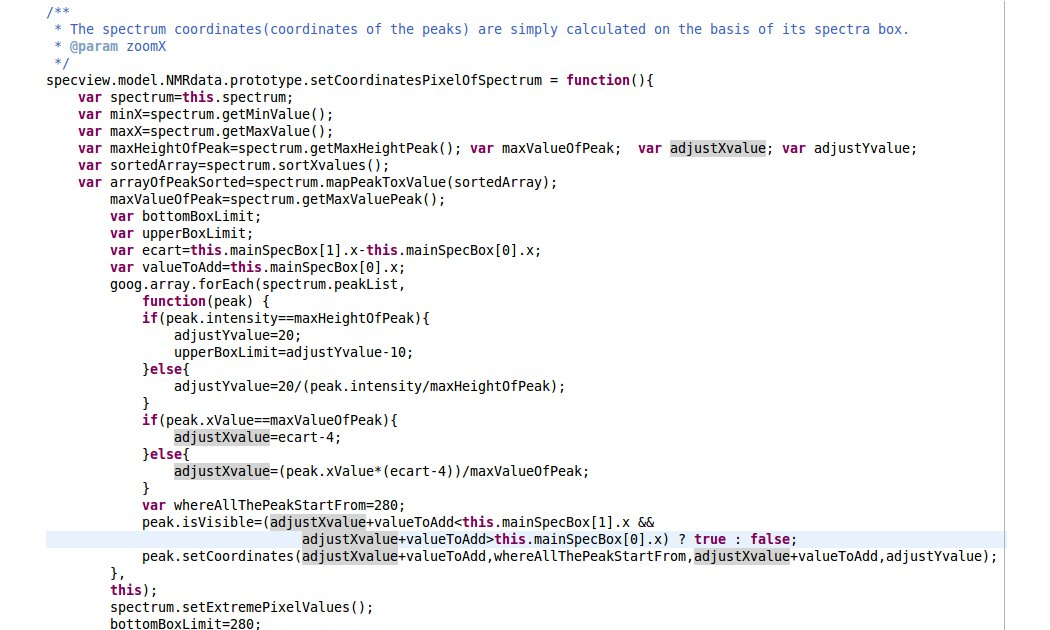
\includegraphics[width=180mm,height=80mm]{./images/setSpecPixel}
%    \label{subd}
    \end{centering}
    \end{figure}

\subsubsection{Mapping}
The viewer has to be interactive. When the user mouse over peaks or atom or bonds, it has to highlights all the objects in relation with the focused object. To do so, we have to create a ``neighborlist'' object.\\

\textbf{The ``neighborlist'' object}

The controller object contains one attribute ``neighborlist''. It is a class for locating the objects nearest to a specified coordinate. That way, when the mouse will hover an object, the controller will know that at this precise coordinate is located an object that has to be highlighted.\\
When we create a ``neighborlist'' object, we create an associative array whose keys are coordinates and value are the object at the given coordinate.
\clearpage
